%%%%%%%%%%%%%%%%%%%%%%%%%%%%%%%%%%%%%%%%%%%%%%
%                insertmeeting
% 1) Title (something creative & funny?)
% 2) Date (MM/DD/YYYY)
% 3) Location (ex. Hagerty High School)
% 4) People/Committees Present 
% 5) Picture 
% 6) Start Time & Stop Time (ex. 12:30AM to 4:30PM)
%%%%%%%%%%%%%%%%%%%%%%%%%%%%%%%%%%%%%%%%%%%%%%
\insertmeeting 
	{Space Coast Meet \#3} 
	{01/08/22}
	{Oviedo High School}
	{Annika, Anouska, Clayton, Falon, James, Jensen, Nathan, Ritam, Rose, Samantha, Lilly}
	{Images/RobotPics/robot.jpg}
	{8:00 - 4:30}
	
\section*{General}
\noindent\hfil\rule{\textwidth}{.4pt}\hfil
\subsection*{Goals}
\begin{itemize}
    \item Reflect upon the successes and failures of meet 3 at Oviedo High school 
    \item Evaluate other teams strategies and consider compatibility
    \item Consider what we learned from the meet 

\end{itemize} 

\noindent\hfil\rule{\textwidth}{.4pt}\hfil

\subsection*{Accomplishments}
The Mechromancers had the third meet of the season January 8th at Oviedo High School, Florida. Our team ranked in 1st place, with 5 wins and 1 loss. The meet was considerably more successful than all the other meets by comparison. Not only did we focus on formulating strategies with the other teams we also had considerably more driver practice. Team spirits were certainly high during this meet especially with our members cheering in the stands for the drive team. However we didn't just cheer on our team, we cheered on all of the teams at the meet, keeping the energy levels high and teams across the stands engaged. This meet we really connected with our alliance partners and made sure to establish strategies to gain the maximum amount of points. Our drive team also practiced everyday for about 2 weeks in order to prepare for the meet. This was vital to our success because Scoopie is reliant on having a compatible driver and operator. They also had plenty of time to practice multiple trials for finding the perfect position for the ducks on the carousel and the perfect speed so that the ducks wouldn’t go flying off. While we were considerably happy with the results of the meet we still feel we can do better with some small improvements on some of the components of our robot. 
- We would like to have our new intake iteration completely finished by the next meet in a week
- We would also like to improve the autonomous program in order to get the maximum amount of points possible.
Unfortunately for this meet we were unable to completely finish our improvements on the intake so they will have to wait to be implemented for the next meet .These improvements will considerably increase the speed and efficiency of Scoopie. We also found during this meet that Scoopie's autonomous may clash with other teams autonomous, therefore during the next meet we will be sure to discuss autonomous capabilities specifics before going into the match. For the next match we would also like to have a more worked out autonomous in order to get the maximum amounts of points working with different varieties of other teams’ programs 
Overall, the experience and knowledge we gained from this meet was extremely valuable! 

 

\begin{figure}[ht]
\centering
\begin{minipage}[b]{.48\textwidth}
  \centering
  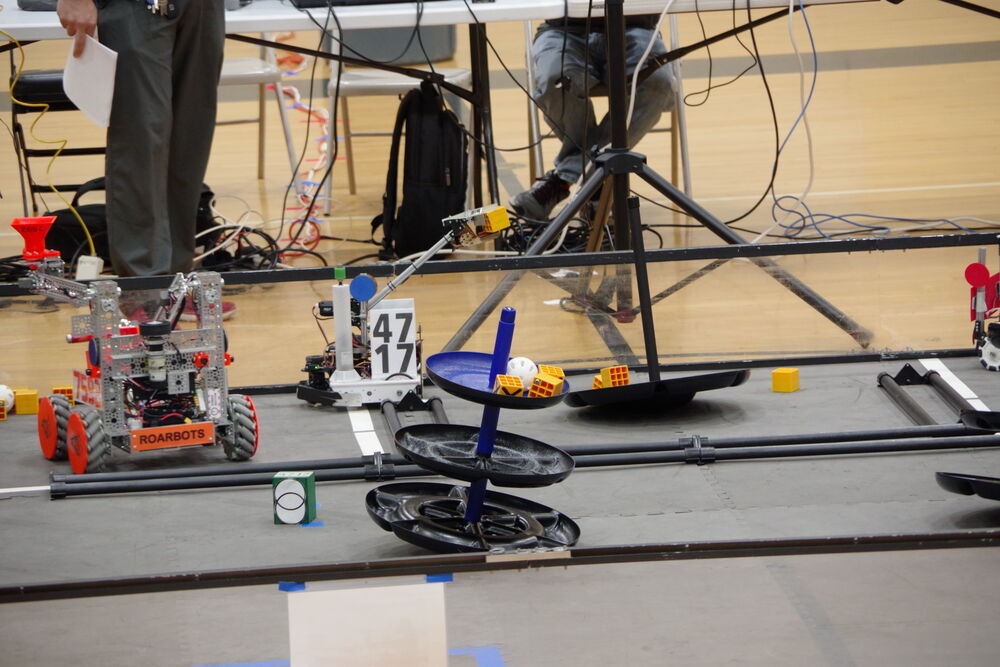
\includegraphics[width=0.95\textwidth]{Meetings/January/01-08-22/1-8-22_Team_Figure1 - Nathan Forrer.JPG}
  \caption{Scoopie in action}
  \label{fig:010822_5}
\end{minipage}%
\hfill%
\begin{minipage}[b]{.48\textwidth}
  \centering
  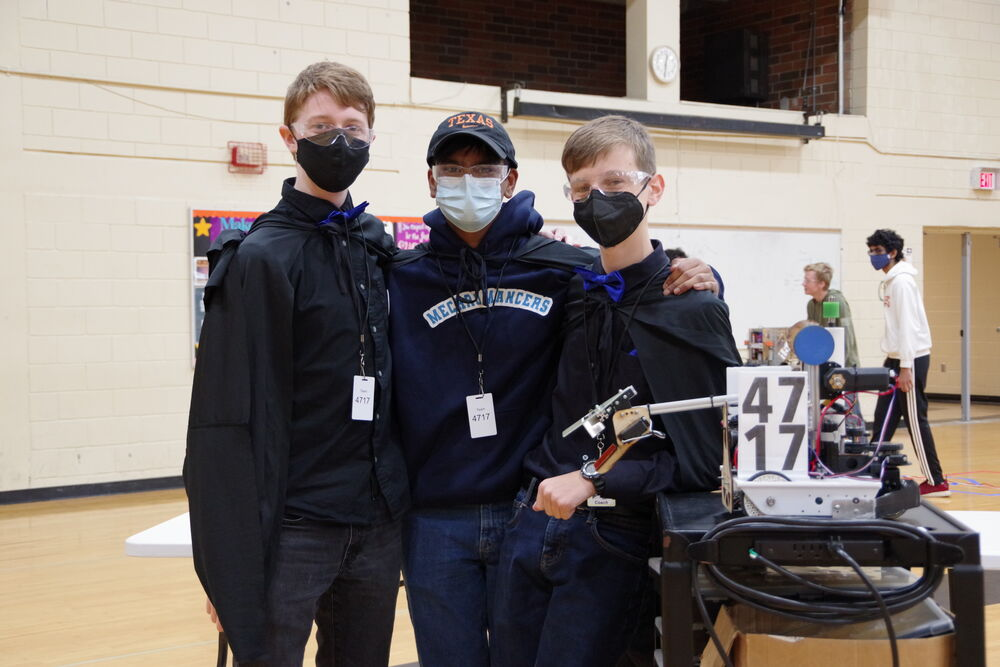
\includegraphics[width=0.95\textwidth]{Meetings/January/01-08-22/1-8-22_Team_Figure2 - Nathan Forrer.JPG}
  \caption{Ritam, Nathan, and Jensen cracking smiles}
  \label{fig:010822_6}
\end{minipage}
\end{figure}

\hhscommittee{Hardware}
\noindent\hfil\rule{\textwidth}{.4pt}\hfil
\subsubsection*{Goals}
\begin{itemize}
    \item Create design for a sweeper intake that will hold blocks better than the roller intake
    \item Make a design that is easy to change and rebuild quickly so we can modify it to be ready for meet 4.


\end{itemize} 

\noindent\hfil\rule{\textwidth}{.4pt}\hfil

\subsubsection*{Accomplishments}
Returning from meet 3, we felt inspired to get working on a new intake. Although our old grabber intake had worked very well with its new changes, we still think  changing to some kind of spinning intake will allWow us to become much more efficient. This type of intake will also make automating cycles in autonomous mode significantly easier for us, as we don't have to decide when to close a clamp, like we would have with the old intake. Instead, with spinner intake we can just turn it on and drive towards the blocks until we sense that we have one. Feeling optimistic, we started discussing the design and how we would overcome issues faced with previous iterations.
The first thing we discussed was how to keep blocks from falling back out the front of the intake when we flip the arm. Because we had faced this issue with our previous roller style intake, we decided to switch our design from a roller to a sweeper, which would have rubber or surgical tubing sticking out of the spinner to hold the blocks in better. With these rubber flaps, we also don't think that having a pivoting arm for the sweeper will be necessary. This will also help us by completely avoiding the problem of having elements fall out due to the roller arm pivoting too high, as we observed with the previous version. To more fully realize some of our ideas we made a sketch of what we expected the intake to  look like (Figure \ref{fig:010822_1}). To out take the blocks, we added a flap on the top of the intake that, after the arm flips over to score, will be on the bottom ready to open up to drop out elements into the hubs.
Moving into onshape, we wanted to make our design as easy to change as possible because of the short amount of time we have before we need the intake to be done. With only a week before meet 4, we need to be able fix any errors without needing to wait for new parts to print for every small adjustment. The way that we plan to get around this is by creating a base that is 3d printed, which connects the intake to the arm. Additionally, we will have laser cut sides that will screw onto the base. This will allow the most highly variable part, the sides, to be redesigned and re cut within minutes because of the speed and ease of laser cutting. We started our cad by creating the base (Figure \ref{fig:010822_2}). From there we created the 2 sides, one of which will hold a super speed servo (Figure \ref{fig:010822_3}). After that, we made the spinner with holes where we can put surgical tubing or rubber (Figure \ref{fig:010822_4}). We are currently unsure of what material we will use for the flaps, but want to test different materials to find what will work best.

 
\begin{figure}[ht]
\centering
\begin{minipage}[b]{.48\textwidth}
  \centering
  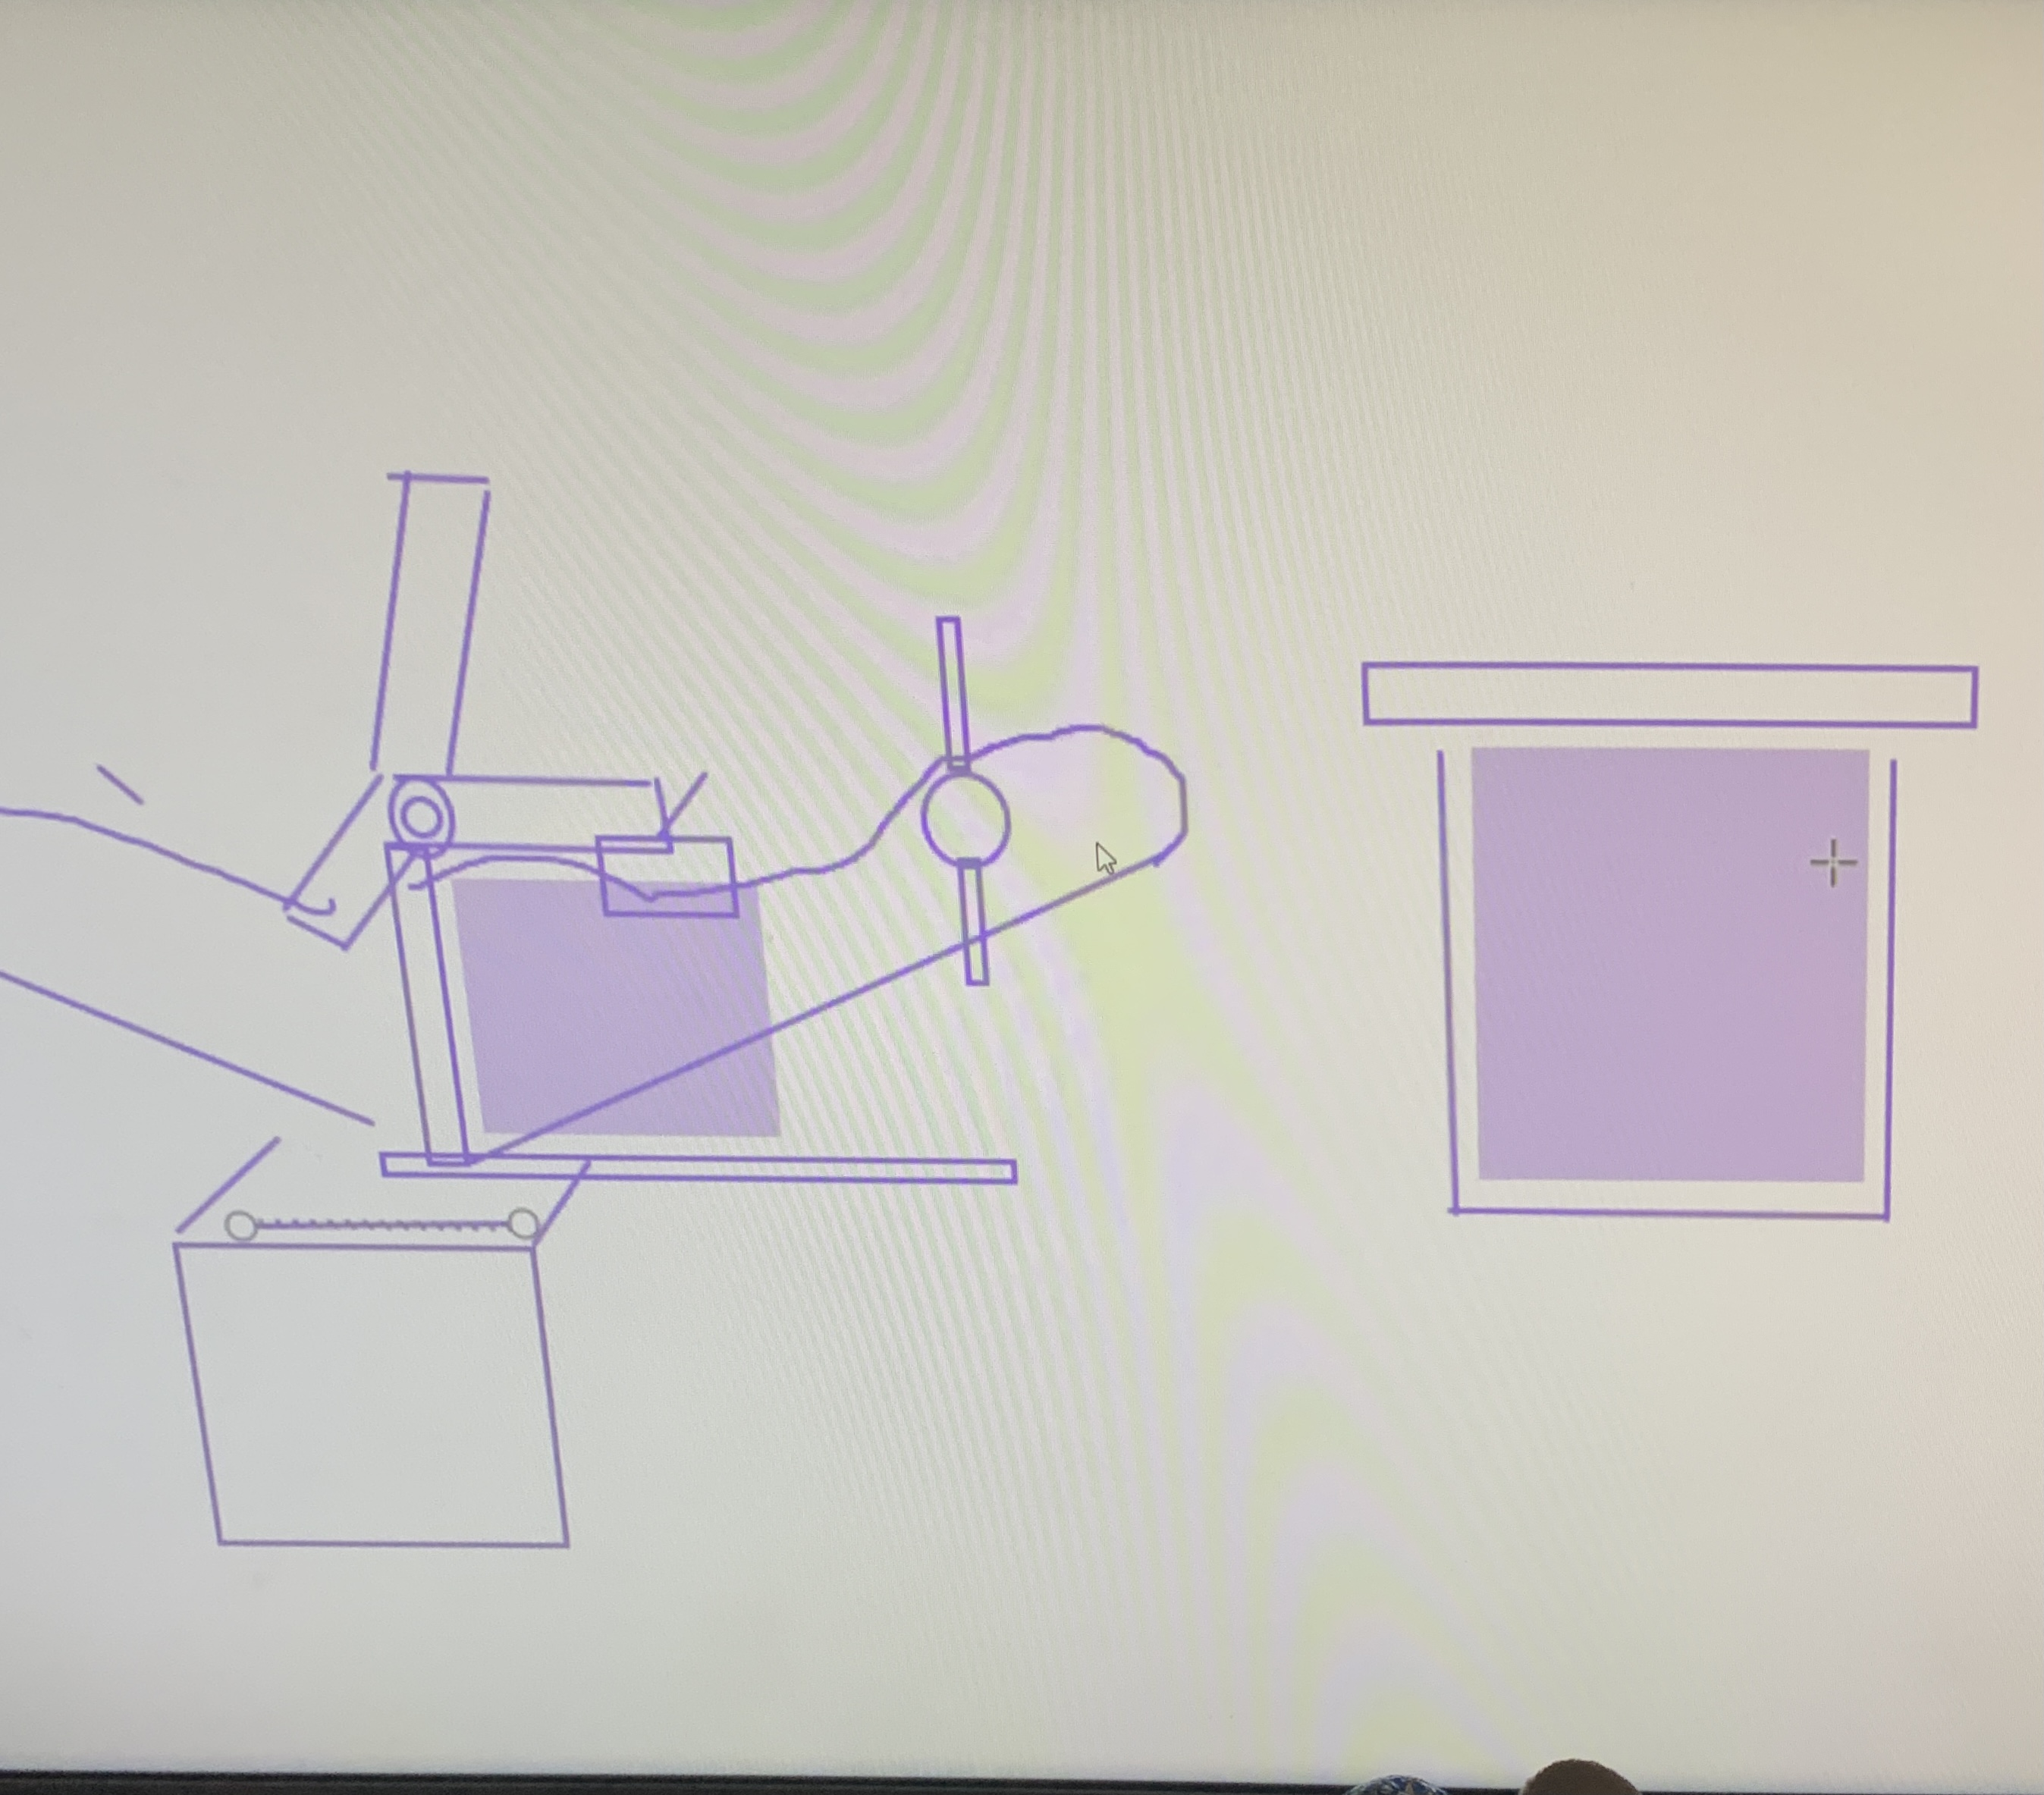
\includegraphics[width=0.95\textwidth]{Meetings/January/01-08-22/1-8-21_CAD_Figure1 - Nathan Forrer.jpg}
  \caption{Intake sketches}
  \label{fig:010822_1}
\end{minipage}%
\hfill%
\begin{minipage}[b]{.48\textwidth}
  \centering
  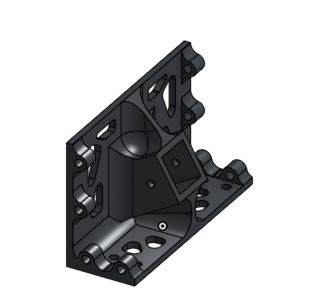
\includegraphics[width=0.95\textwidth]{Meetings/January/01-08-22/1-8-21_Hardware_Figure2 - Nathan Forrer.JPG}
  \caption{The new intake base}
  \label{fig:010822_2}
\end{minipage}
\end{figure}


\begin{figure}[ht]
\centering
\begin{minipage}[b]{.48\textwidth}
  \centering
  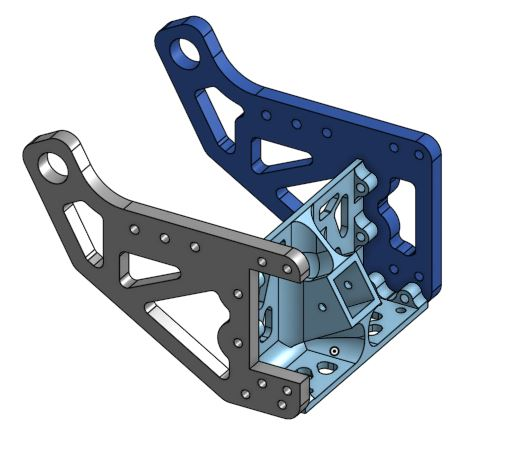
\includegraphics[width=0.95\textwidth]{Meetings/January/01-08-22/1-8-21_Hardware_Figure3 - Nathan Forrer.JPG}
  \caption{The dual servo holder}
  \label{fig:010822_3}
\end{minipage}%
\hfill%
\begin{minipage}[b]{.48\textwidth}
  \centering
  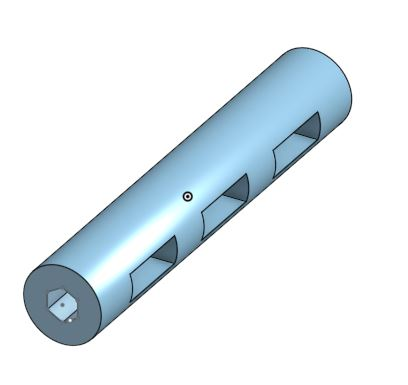
\includegraphics[width=0.95\textwidth]{Meetings/January/01-08-22/1-8-21_Hardware_Figure4 - Nathan Forrer.JPG}
  \caption{The new custom spinner}
  \label{fig:010822_4}
\end{minipage}
\end{figure}


\whatsnext{
\begin{itemize}
    \item complete and use our new intake
allow more time for software to work on autonomous

\end{itemize} 
}


